In this chapter, we discuss the concept of regression and related methods and
the role they play in predicting future housing prices. Regression analysis is a
statistical technique used to determine the contributing effect of a set of
explanatory variables on the response variable.

\section{Quantitative Measures of Performance}
Selecting the best method among many different statistical learning approaches
can be one of the practitioners' most daunting tasks.  One particular approach
may work best on a particular data set, but some other methods may perform
better on a similar but different data set.
Therefore, it is critical to select which method produces the best results for
any given data set.

To assess a particular model's predictive performance on a given data set, we
need some way to measure how well its predictions match the observed data.
\subsection{Mean Squared Error}
When
an outcome is a number (regression problem), the most commonly used method for
characterizing a model's predictive capabilities is to use the mean squared
error (MSE), which is:
\begin{eqnarray}
    \label{eqn:mse}
    MSE = \frac{1}{n} \sum_{i=1}^{n}(y_i - \hat{f}(x_i))^2
\end{eqnarray}
where $\hat{f}(x_i)$ is the prediction that $\hat{f}$ gives for the $i_{th}$
observation. If the predicted responses are very close to the actual responses,
the MSE will be small and vice versa.

\subsection{Coefficient of Determination}
We also use the coefficient of determination ($R^2$) to measure the proportion
of the information in the data explained by the model.  For example, an $R^2$
value of 0.8 means that the model can explain  80 percent of the outcome's
variation. An $R^2$ of 1 indicates that the regression predictions perfectly fit
the data. It should be noted that $R^2$ is a measure of correlation, not
accuracy.

\noindent $R^2$ is calculated as the correlation coefficient between the
observed and predicted values and squares it:
\[ R^2 = 1 - \frac{SS_{res}}{SS_{tot}}\]
where $SS_{res}$ is the sum of squares of residuals and $SS_{tot}$ is the total
sum of squares (proportion to the variance of the data)

\section{The Problem of Overfitting}
\label{sec:overfitting}
New technologies have changed how we collected data in various fields as diverse
as finance, commerce, and medicine in recent years.  It is not unusual to obtain
an almost unlimited number of feature measurements. We might expect it will always be better to use as many features as possible in
our model. In other words, we suppose that the best model is the most flexible
one. However, this is not always the case.  Fitting a  model with a large number
of features can lead to overfitting the data, which means that the model follows
the errors or noise too closely.  This type of model will usually have poor
accuracy when predicting a new sample.

To prevent overfitting, in this study we use less flexible fitting methods such
as penalized regression models as explained in
\ref{sec:penalized_regression_models}


\section{Linear Regression}
\label{sec:linear-regression}

Linear regression is a straightforward approach for supervised learning. In
particular, linear regression is a useful tool for predicting a quantitative
response. Linear regression has been around for a long time and is the topic of
numerous works of literature.  Linear regression can represent more than one
variable as input, but all the variables are linear correlated. This is in line
with the Hedonic Price Theory, which asserts that a product's price can be
regarded as a function of the measurable,utility-affecting attributes or
characteristics of the product \parencite{rosen1974hedonic}

According to hedonic pricing theory, an Airbnb accommodation listing is a bundle
of factors that impact the overall product's quality and provide consumers with
value and satisfaction.  Accordingly, a listing's price can be linked to the
presence or absence of specific items; it is a price proposal reflecting the
host's assumptions about implicit marginal prices of particular listing
characteristics.

The aim of ordinary least squares linear regression is to find the plane that
minimizes the sum-of-squared errors between the observed and predicted
response.
\begin{eqnarray}
SSE = \sum_{i=1}^{n}(y_i - \hat{y}_i)^2
\end{eqnarray}
where $y_{i}$ is the outcome and $\hat{y}_i$ is the model prediction of that
sample’s outcome.
It can be proven mathematically  that the optimal plane is
\begin{eqnarray}
    \label{eqn:optimal_plane}
    (X^TX)^{-1}X^{T}y
\end{eqnarray}
where \textbf{X} is the matrix of predictors, and y is the response vector.
Equation ~\ref{eqn:optimal_plane} is also known as $\hat{\beta}$ (“beta-hat”) in statistical texts
and is a vector that comprises the parameter estimates or coefficients for each
predictor. This quantity (~\ref{eqn:optimal_plane}) is easy to compute, and the coefficients are directly
interpretable

Given some minimal premises about the distribution of the residuals \footnote{
the error terms $\epsilon$ are independent, uncorrelated and normally
distributed with mean of zero and constant variance $\sigma^2$ (a.k.a.
homoskedasticity)}, it has conclusively been shown that the parameter estimates
that minimize SSE are the ones that have the least bias of all possible
parameter estimates (\textcite{graybill1976theory} ). Therefore, these estimates
minimize the bias element of the bias-variance trade-off.

In linear regression, overfitting is more likely to be a serious concern
\parencite{harrell2015regression}. When
there is little or no theory available to guide on selecting the predictors, we
want to include in our model as many features as possible. However, we run the
risk of including irrelevant features that actually have no relation to the
dependent variable being predicted, thus might not improve the prediction
performance.

\section{Penalized Regression Models}
\label{sec:penalized_regression_models}

Penalized regression models shrink the size of multiple linear regression
coefficients, thus introducing bias, while attempting to improve the prediction.

\subsection{Ridge Regression}

%Originally proposed in 1970 by Arthur E. Hoerl and Robert W. Kennard, ridge
%regression attempts to correct for overfitting through regularization.
When the model overfits the data or issues with collinearity,
the linear regression parameter estimates may become inflated.  We want to find
a method to control the magnitude of these estimates to reduce the SSE.
One possible solution is to use Ridge Regression (\textcite{hoerl1970ridge})  to
control (or regularize) the parameter estimates by adding a penalty to the SSE
if the estimates become large.
%by adding a penalty on the sum of the squared
%regression parameters, often called L2 parameter.

Ridge regression is very similar to least squares, except that the coefficients
ridge are estimated by minimizing a slightly different quantity. In particular,
the ridge regression coefficient estimates $\hat{\beta}^R$ are the
values that minimize:
\begin{eqnarray}
    \label{eqn:ridge-optimal}
    \sum_{i=1}^{n}(y_i -\beta_0 - \sum_{j=1}^{p}\beta_j x_{ij}) ^ 2 + \lambda
    \sum_{j=1}^{p}\beta_{j}^2 = RSS + \lambda \sum_{j=1}^{p}\beta_{j}^2
\end{eqnarray}
In  Equation  ~\ref{eqn:ridge-optimal} we made a trade-off between two different
criteria. As with least squares, ridge regression seeks coefficient estimates
that fit the data well, by making the RSS small. But, the second term, $\lambda
\sum_{j=1}^{p}\beta_{j}^2$ signifies that a second-order penalty (i.e., the
square) is being used on the parameter estimates.
This shrinkage penalty is small when $\beta_1$,...,$\beta_p$ are close to zero,
and so it has the effect of shrinking penalty the estimates of $\beta_j$ towards
zero.

When $\lambda = 0$, the penalty term has no effect, and ridge regression is the same
as least squares estimates. However, as $\lambda \to \infty$, the influence of
the shrinkage penalty increases, and the ridge regression will shrink the
estimates towards  zero.
In contrast to least squares, which produces only one set of coefficient
estimates, ridge regression will generate a different set of coefficient
estimates, $\hat{\beta}_{\lambda} ^ {R}$, for each value of $\lambda$.

\subsection{Lasso Regression}
One drawback of ridge regression that it does not shrink any of the parameter
estimates towards 0. Therefore, the model does not conduct feature selection.

\noindent Least Absolute Shrinkage and Selection Operator (Lasso)
\parencite{tibshirani1996regression} model is a modern
alternative to ridge regression that overcomes this disadvantage. The name comes
from its functionality that it does not only shrink coefficients towards zero,
but it also performs feature selection.


The lasso  coefficients, $\hat{\beta}^L$ , minimize the quantity:
\begin{eqnarray}
    \label{eqn:lasso-optimal}
    \sum_{i=1}^{n}(y_i -\beta_0 - \sum_{j=1}^{p}\beta_j x_{ij}) ^ 2 + \lambda
    \sum_{j=1}^{p} \mid \beta_{j} \mid= RSS + \lambda \sum_{j=1}^{p} \mid \beta_{j} \mid
\end{eqnarray}
Notice that the lasso and ridge regression have similar formulations. The only distinction is in the penalty term. In particular, the $\beta_j^2$ term in the ridge regression penalty (6.5) has been replaced by $\mid \beta_{j} \mid$ in the lasso penalty
The implication of this modification is that penalizing the absolute values has the effect of setting some of the coefficient estimates to be exactly equal to zero for some value of $\lambda$. Thus the lasso yields models that simultaneously use regularization to improve the model and to conduct feature selection.

We can formulate the lasso and ridge regression coefficient estimates in
\ref{eqn:lasso-optimal} and \ref{eqn:ridge-optimal} as solving following
problems:

\begin{equation}
    \label{eqn:ridge-optimal}
    \begin{aligned}
    \min_{\beta} \quad \sum_{i=1}^{n}(y_i -\beta_0 - \sum_{j=1}^{p}\beta_j
    x_{ij}) ^ 2  \quad \textrm{subject to} \quad \sum_{j=1}^{p}\mid\beta_j\mid
    \leq s
    \end{aligned}
\end{equation}
and
\begin{equation}
    \label{eqn:lass-optimal}
    \begin{aligned}
    \min_{\beta} \quad \sum_{i=1}^{n}(y_i -\beta_0 - \sum_{j=1}^{p}\beta_j
    x_{ij}) ^ 2  \quad \textrm{subject to} \quad \sum_{j=1}^{p}\beta_j^2\leq s
    \end{aligned}
\end{equation}

In the figure \ref{fig:feature-selection}, we illustrate why the lasso performs
feature selection, while ridge regression does not.To simplify the problem, we
consider only two parameters $\beta_1$ and $\beta_2$.
The elliptic centered around $\hat{\beta}$ are contours of the sum of squares
error with the OLS estimator in the center. All of the points on a given ellipse
has the same value of RSS. The diamond and circle represent the lasso and ridge
regression constraints in \ref{eqn:lasso-optimal} and \ref{eqn:ridge-optimal}.

The lasso and ridge regression coefficient estimates are the first point at
which an ellipse touches the constraint set.
Note that the ridge regression has a circular constraint with no sharp points.
This intersection will not generally occur on an axis. So the ridge regression
coefficient estimates will be exclusively non-zero. However, the lasso
constraint has corners at each of the axes, and so the ellipse will often
intersect the constraint region at an axis. When this occurs, one of the
coefficients will equal zero.In this way, the lasso performs \textit{feature
selection}.
\begin{figure}[H]\centering
    \caption{Illustration of two dimensional case of estimation for the lasso
    (right) and the ridge regression}
    \label{fig:feature-selection}
    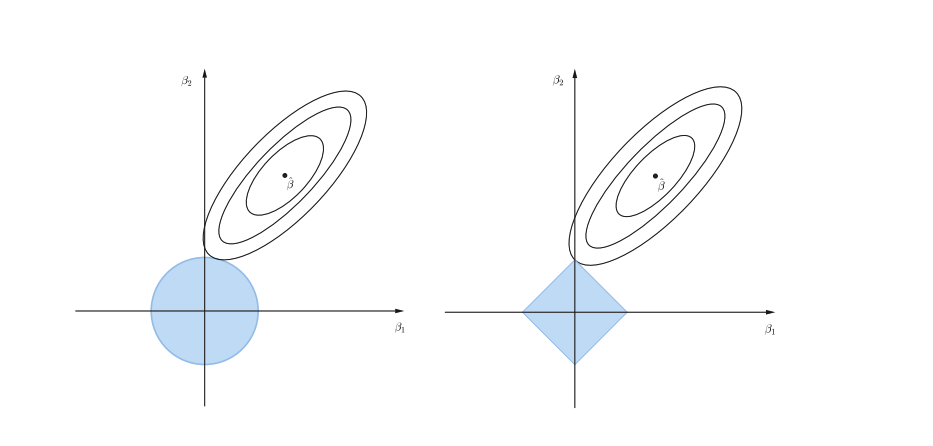
\includegraphics[width=\textwidth]{feature-selection.png}
\end{figure}
\vspace{1mm}
\subsection{Selecting the Tuning Parameter}

Choosing an optimized value of tuning parameter $\lambda$ is critical when
implementing the ridge and the lasso regression.
We do not want to choose $\lambda$ too small due to the low restriction. On the
other hand, when $\lambda$ is very large, the restriction is more substantial
than it is desired. We handle the problem of the optimal value of  by using a
cross-validation technique. \textcite{efron1994introduction} introduce the algorithm, which describes
the procedure of cross-validation.

\begin{algorithm}[H]
\setstretch{1.35}
\SetAlgoLined
\renewcommand{\labelenumi}{(\Roman{enumi})}
Split the data into K roughly equal-sized parts.

For the $k^{th}$ part, fit the model to the other K − 1 parts of the data, and
calculate the mean squared error of the fitted model when predicting the
$k^{th}$ part of the data.

Repeat step 2 for k = 1, 2, . . . , K and average the K estimates of mean
squared error $MSE_1$, $MSE_2$,..., $MSE_k$.

For each tuning parameter value $\lambda$, compute the average error over all
folds \[CV_{(k)} = \frac{1}{k} \sum_{i=1}^{k} MSE_i\]

 \caption{K-Fold Cross Validation}
\end{algorithm}


We choose a grid of $\lambda$ values and calculate the cross-validation error
for each value of $\lambda$. We then select the tuning parameter value for which
the cross-validation error is smallest.


\section{XGboost}

All the approaches reviewed so far suffer from the fact that they use a single
model for predicting the response variable. Hence the ability to choose a
suitable model is crucial to have any chance to obtain good results.

\noindent Machine Learning practitioners have to consider many factors such as
the quantity of data, the dimensionality of the space, and distribution
hypothesis to find a high predictive power model.

Using this approach, we have to face the bias-variance tradeoff. On the one
hand, we want our model to have enough degrees of freedom to resolve the
underlying complexity of the data we are working with. On the other hand, we
also want it to have not too many degrees of freedom to avoid high variance and
be more robust.

Boosting, on the other hand, takes a more iterative approach. It is an ensemble
technique in which several models are combined to achieve a better one.

\subsection{Ensemble Methods}

Imagine we want to buy a new laptop. We are unlikely to walk into a store and
buy a laptop. You search the product on the internet, read reviews, compare
models, prices. We ask for opinions from our family and friends. In brief, we
investigate, seek the \textit{wisdom of the crowd} before making an informed
decision.\newline
Likewise, if we combine multiple learning algorithms, we will often obtain
better predictions than the best individual algorithm. We call a group of
predictors an \textit{ensemble}, and the technique is called Ensemble Learning. The
Ensemble Learning algorithm is called an Ensemble method.

In practice, two ensemble models have proven to be effective on a wide range of
datasets for classification and regression, both of which use decision trees as
their building blocks: random forests and gradient boosted decision trees.

%\subsection{Boosting}
\subsection{Gradient Boosting}

While there are several boosting methods available, the two most popular are
Adaptive Boosting \autocite{freund1997decision} and Gradient
Boosting \autocite{friedman2001greedy}. In this study, we focus on Gradient
boosting trees and its high-performance implementation, XGBoost.
The Gradient boosting trees model uses a regression tree as the base learner.
\citeauthor{kuhn2013applied} \parencite{kuhn2013applied} suggests three reasons
why trees make an excellent base learner for boosting:
\begin{enumerate}
    \item By limiting their depth, they can be weak learners.
    \item We can add together separate trees easily.
    \item Trees can be created quickly.
\end{enumerate}

The basic gradient boosting regression principles are: given mean squared error
( a loss function ) and regression trees (weak learners). The goal of Gradient
Boosting Trees is to find an additive model that minimizes the loss function.

We illustrate this approach in Figure ~\ref{fig:gradient-boosting-illustration}

\begin{figure}[H]\centering
    \caption{Gradient Boosting Approach}
    \label{fig:gradient-boosting-illustration}
    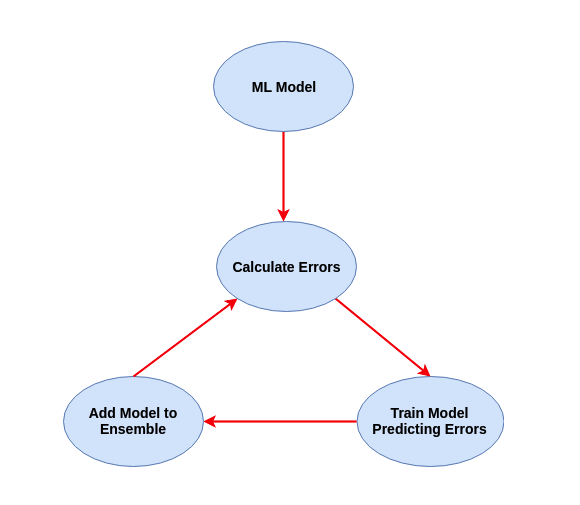
\includegraphics[width=\textwidth]{gradient-boosting-illustration.png}
\end{figure}

\textcite{kuhn2013applied} illustrate the Gradient Boosting for
Regression algorithm as followed:

\begin{algorithm}[H]
\setstretch{1.35}
\SetAlgoLined

\renewcommand{\labelenumi}{(\Roman{enumi})}
Select tree depth, D, and number of iterations, K

Compute the average response, $\bar{y}$, and use this as initial predicted value for each sample

\For{$k\gets0$ \KwTo $K$ }{
    Compute the residual, the difference between observed value and the \textit{current} predicted value, for each sample

    Fit a regression tree of depth, D, using the residuals as the response

    Predict each sample using regression fit in the previous step

    Update the predicted value of each sample by adding the previous iteration's predicted value to the predicted value generated in the previous step

    }
 \caption{Simple Gradient Boosting for Regression}
\end{algorithm}
\subsection{XGBoost}
Extreme Gradient Boosting (XGBoost) is a variant of the gradient tree boosting.
Gradient boosting and XGBoost follows the same principle. The key differences
between them lie in implementation details.
Specifically, features of XGBoost which make it stand out of from the rest of
other gradient boosting algorithms, are
\begin{itemize}
    \item Clever penalization of trees
    \item A proportional shrinking of leaf nodes
    \item Newton Boosting
    \item Extra randomization parameter
    \item Implementation on single, distributed systems and out-of-core computation
\end{itemize}
%Several reasons explain why XGBoost is popular in the machine learning
%community, which includes:
Besides these superior features, there are other reasons why XGBoost is getting
popular in the machine learning community:
\begin{itemize}
    \item Can solve a wide range of applications such as regression,
        classification, ranking, and user-defined prediction problems.
    \item Portability: Runs smoothly on Windows, Linux, and OS X.
    \item Languages: Supports all major programming languages, including C++,
        Python, R, Java, Scala, and Julia.
    \item Cloud Integration: Supports AWS, Azure, and Yarn clusters and works
        well with Flink, Spark, and other ecosystems.
\end{itemize}

Since its introduction in 2014, this algorithm has
been credited with winning numerous Kaggle competitions and being the driving
force under the hood for several cutting-edge industry applications. Futhermore,
XGBoost has been shown to provide state-of-the-art results for diverse problems,
including web text classification, customer behavior prediction, motion
detection, and malware classification \textcite{chen2016xgboost}
\textcite{nielsen2016tree}.

While XGBoost is suitable for predicting, it does so at the expense of its
interpretability.  As shown in Figure
\ref{fig:flexibility-interpretability-tradeoff}, compared to restrictive models
such as Lasso or Least Squares, Boosting is a highly flexible (complex) approach
that is harder to interpret.

\begin{figure}[H]\centering
    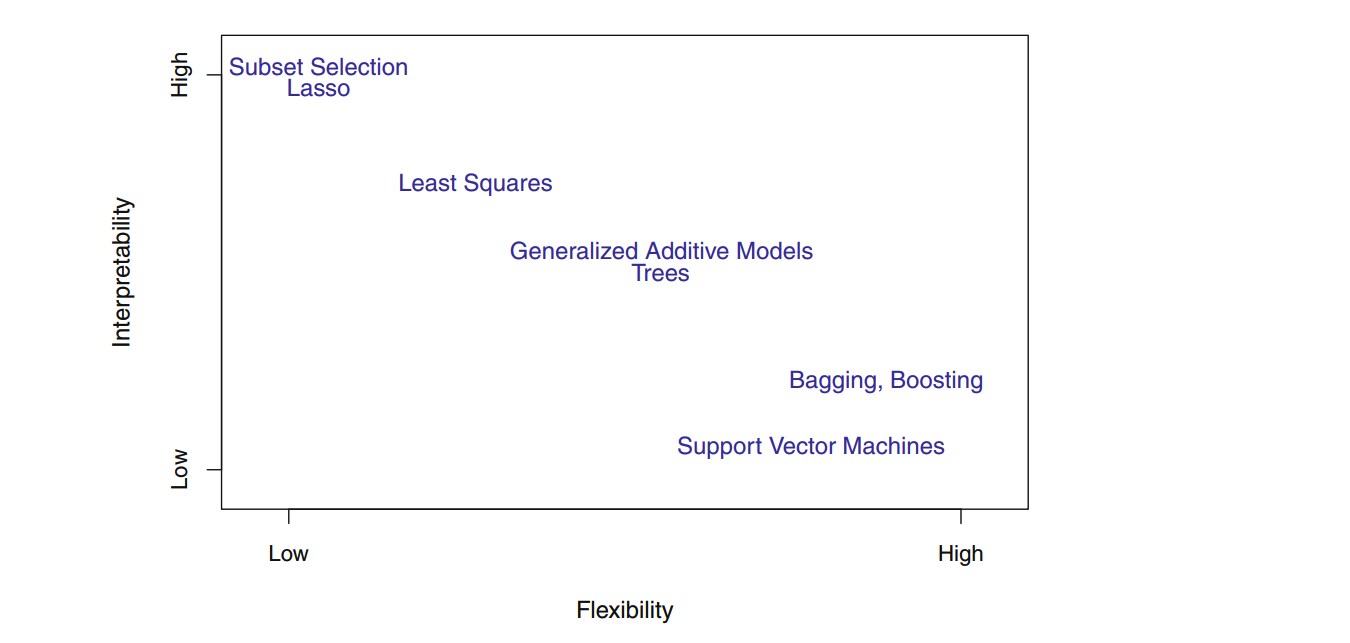
\includegraphics[width=0.75\textwidth]{flexibility-interpretability-tradeoff.png}
    \caption{Interpretability and Flexibility Tradeoff}
    \label{fig:flexibility-interpretability-tradeoff}
    \source{\textcite{james2013introduction}}
\end{figure}
